\documentclass[12pt]{article}
\usepackage[english]{babel}
\usepackage{enumerate, setspace, float, stackengine}
\usepackage[hidelinks]{hyperref}
\usepackage[margin=1.5cm]{geometry}
\usepackage{caption, subcaption}
\usepackage{amsmath, amsfonts, amssymb}
\usepackage{fontspec}   %加這個就可以設定字體
\usepackage{xeCJK}       %讓中英文字體分開設置
\setCJKmainfont{標楷體} %設定中文為系統上的字型,而英文不去更動,使用原TeX字型

\title{\textbf{Digital Speech Processing}\\ Homework 1 - HMM}

\author{R04922058 鄭以琳}
\date{\large \today}


\begin{document}
\maketitle

\section{Execution Environment}
    \begin{itemize}
        \item \textbf{Environment:} \\
            Linux Ubuntu X86\_64
        \item \textbf{Compile:}\\
            \verb|$ make clean| \\
            \verb|$ make all|
        \item \textbf{Execute:}\\
            \verb|$ ./train  iteration  model_init.txt  seq_model_01.txt  model_01.txt| \\
            \verb|$ ./test  modellist.txt  testing_data.txt  result.txt|
    \end{itemize}

\section{Result}
    \begin{itemize}
        \item \textbf{Parameters:} \\
            \# Iteration = 2000 \\
            Initial model = \verb|model_init.txt|
        \item \textbf{Accuracy:}\\
            Accuracy of \verb|testing_data1.txt| = 0.8696
    \end{itemize}

\section{Experiment}
    I built the models with different numbers of iterations and calculate the accuracy of \verb|testing_data1.txt|.\\
    The result is shown below:\\
    \begin{table}[h!]
        \centering
        \label{tbl:accuracy}
        \begin{tabular}{|c|c|c|c|c|c|c|c|c|c|c|c|}
        \hline
        \textbf{\# Iterations} & 10    & 50   & 100 & 300   & 500  & 1000  & 1500 & 2000  & 2500 & 3000  & 3500  \\ \hline
        \textbf{Accuracy}      & 54.08 & 82.8 & 81  & 84.88 & 85.6 & 86.96 & 87   & 86.96 & 86.8 & 86.76 & 86.76 \\ \hline
        \end{tabular}
    \end{table}
    \begin{figure}[H]
        \centering
        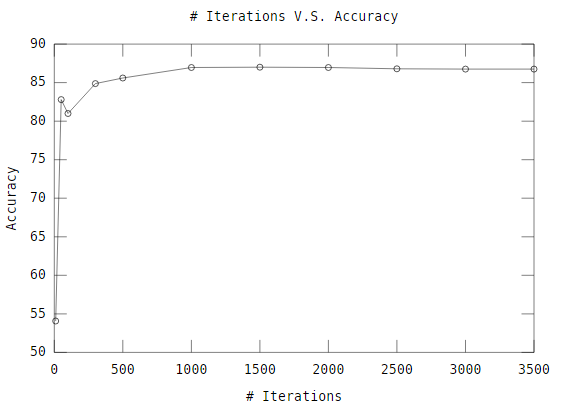
\includegraphics[width=0.8\textwidth]{fig}
        \label{fig:accuracy}
    \end{figure}

 
\end{document}
